\section{Pruebas}
Para comprobar el funcionamiento del programa, se ingreso la siguiente función, en un archivo con una frecuencia de muestreo de 44100 muestras/s. \\ cos(2*pi*t*(exp(log(20)+n/N*6.6))):
\begin{figure}[H]
	\centering
	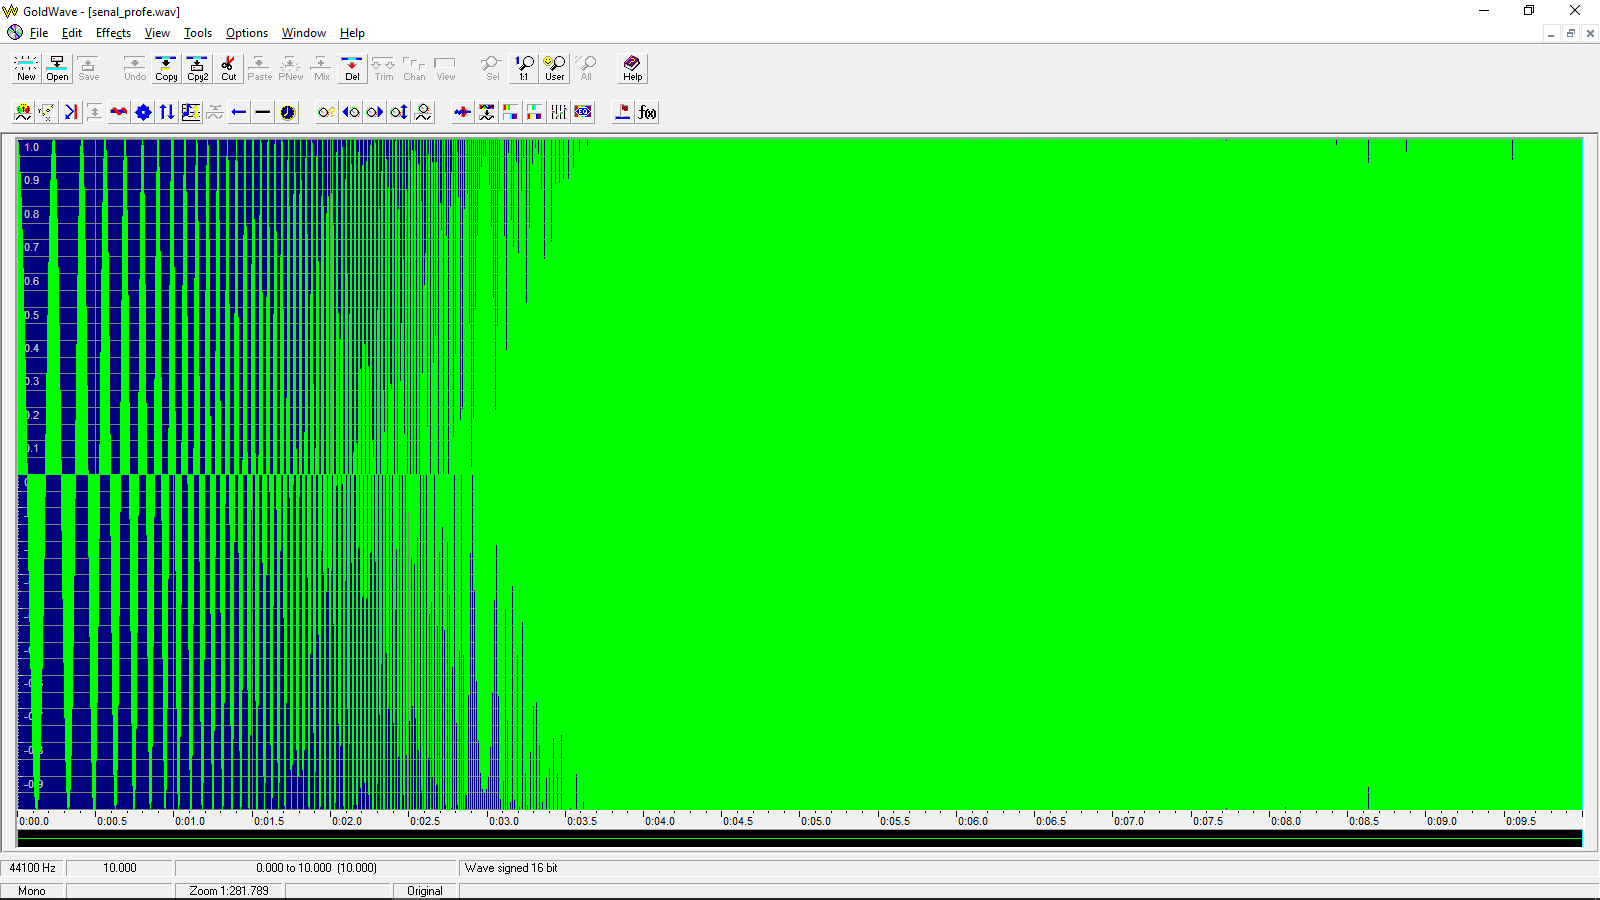
\includegraphics[scale=.35]{img/entrada1.png}
	\caption{Entrada 1}
	\label{fig:prueba1}		
\end{figure}
Al realizar la convolución mediante el uso del programa, se obtuvo la siguiente salida:
\begin{figure}[H]
	\centering
	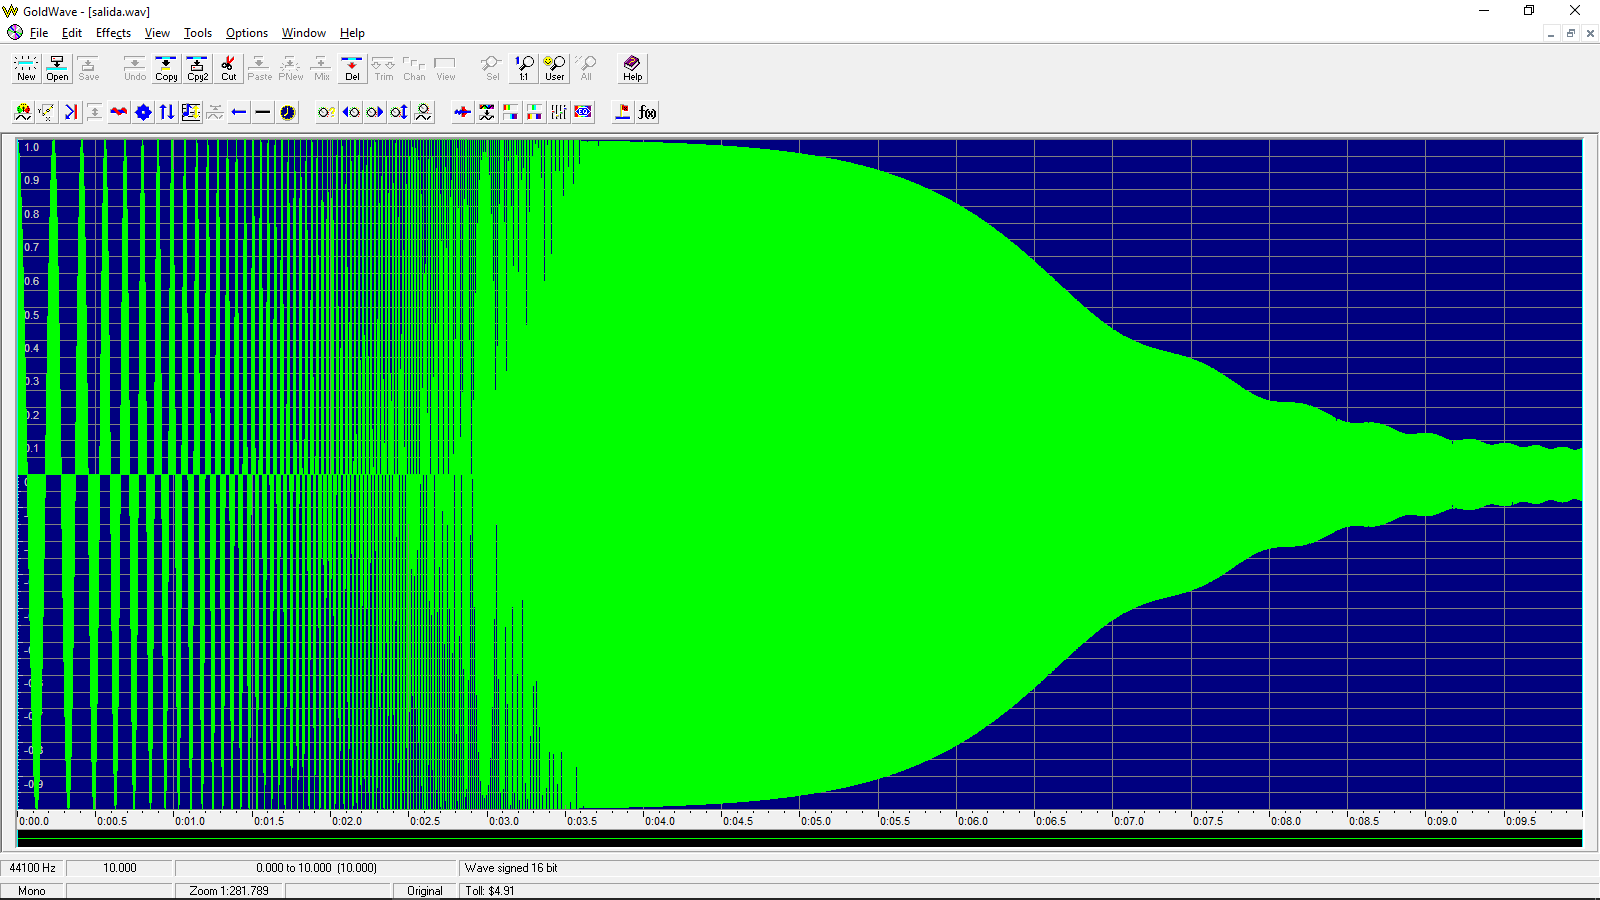
\includegraphics[scale=.35]{img/salida1.png}
	\caption{Salida 1 - 20 coeficientes en el filtro}
	\label{fig:salida1}		
\end{figure}
Como se observa, la señal de salida es igual a la señal de entrada con la diferencia que cuando se alcanza la frecuencia de 1000Hz en la señal de salida, la amplitud de la misma empieza a decaer hasta aproximarse a cero.\\ En la Figura 5, se observa la frecuencia que tiene la señal al momento de que esta decae 3dB o su amplitud es .707 veces la amplitud de la señal original. Esta frecuencia es la frecuencia de corte del filtro RC.
\begin{figure}[H]
	\centering
	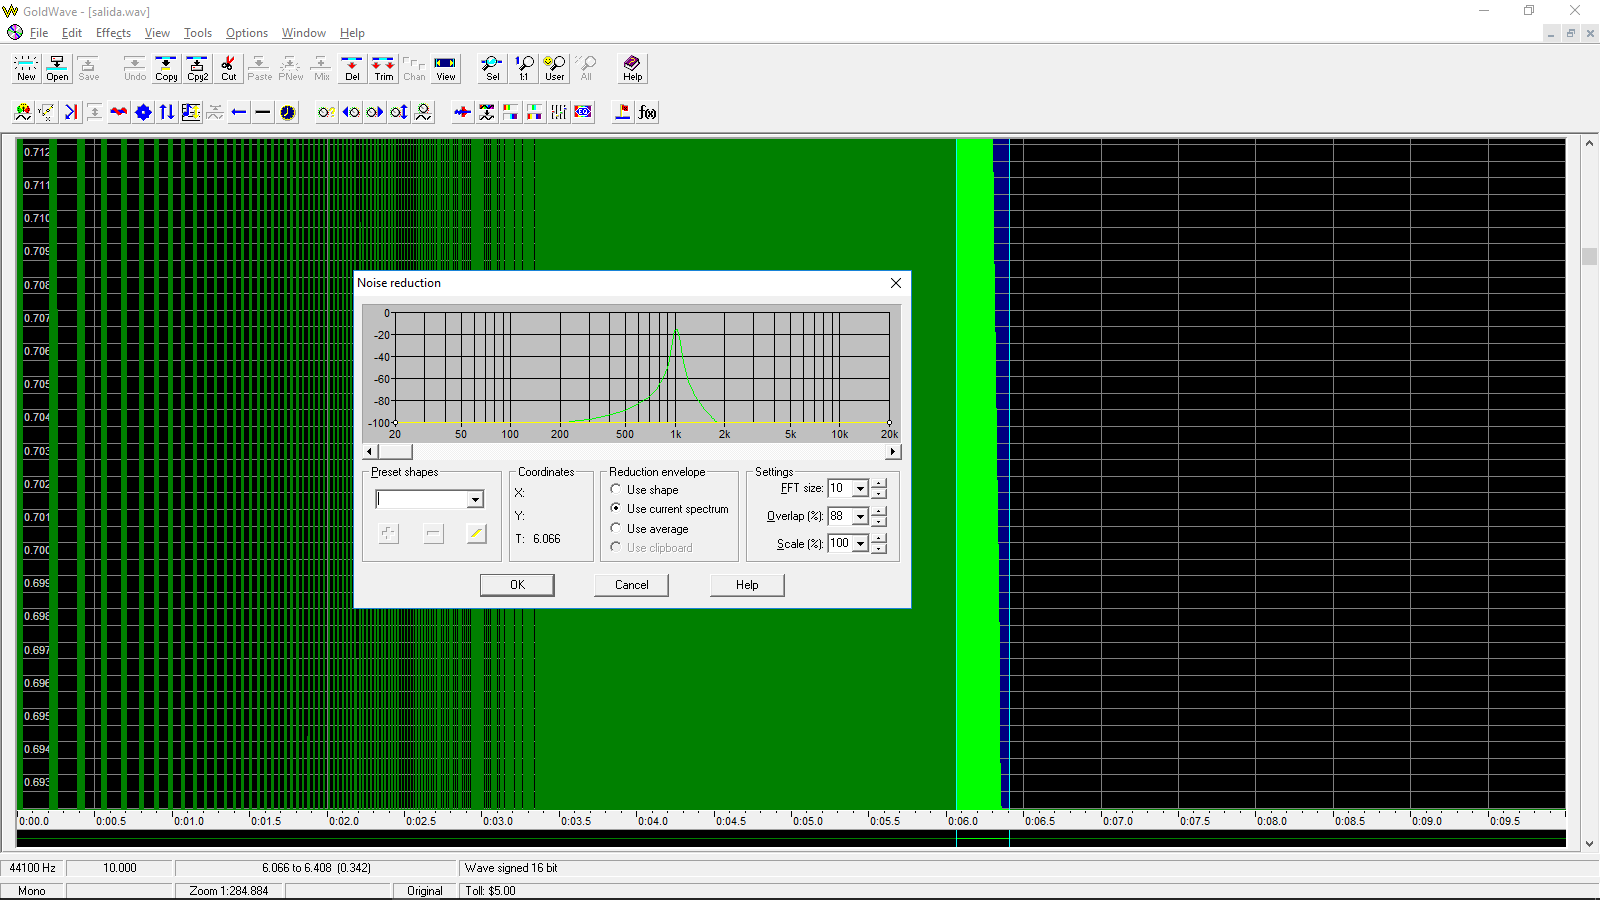
\includegraphics[scale=.4]{img/fc.png}
	\caption{Frecuencia de corte donde la señal decae 3dB}
	\label{fig:fc}		
\end{figure}
La salida mostrada en la Figura 4, fue obtenida calculando solo 20 coeficientes para el filtro. A continuación se anexan dos Figuras más, en donde se usan 30 y 40 coeficientes para el filtro respectivamente.
\begin{figure}[H]
	\centering
	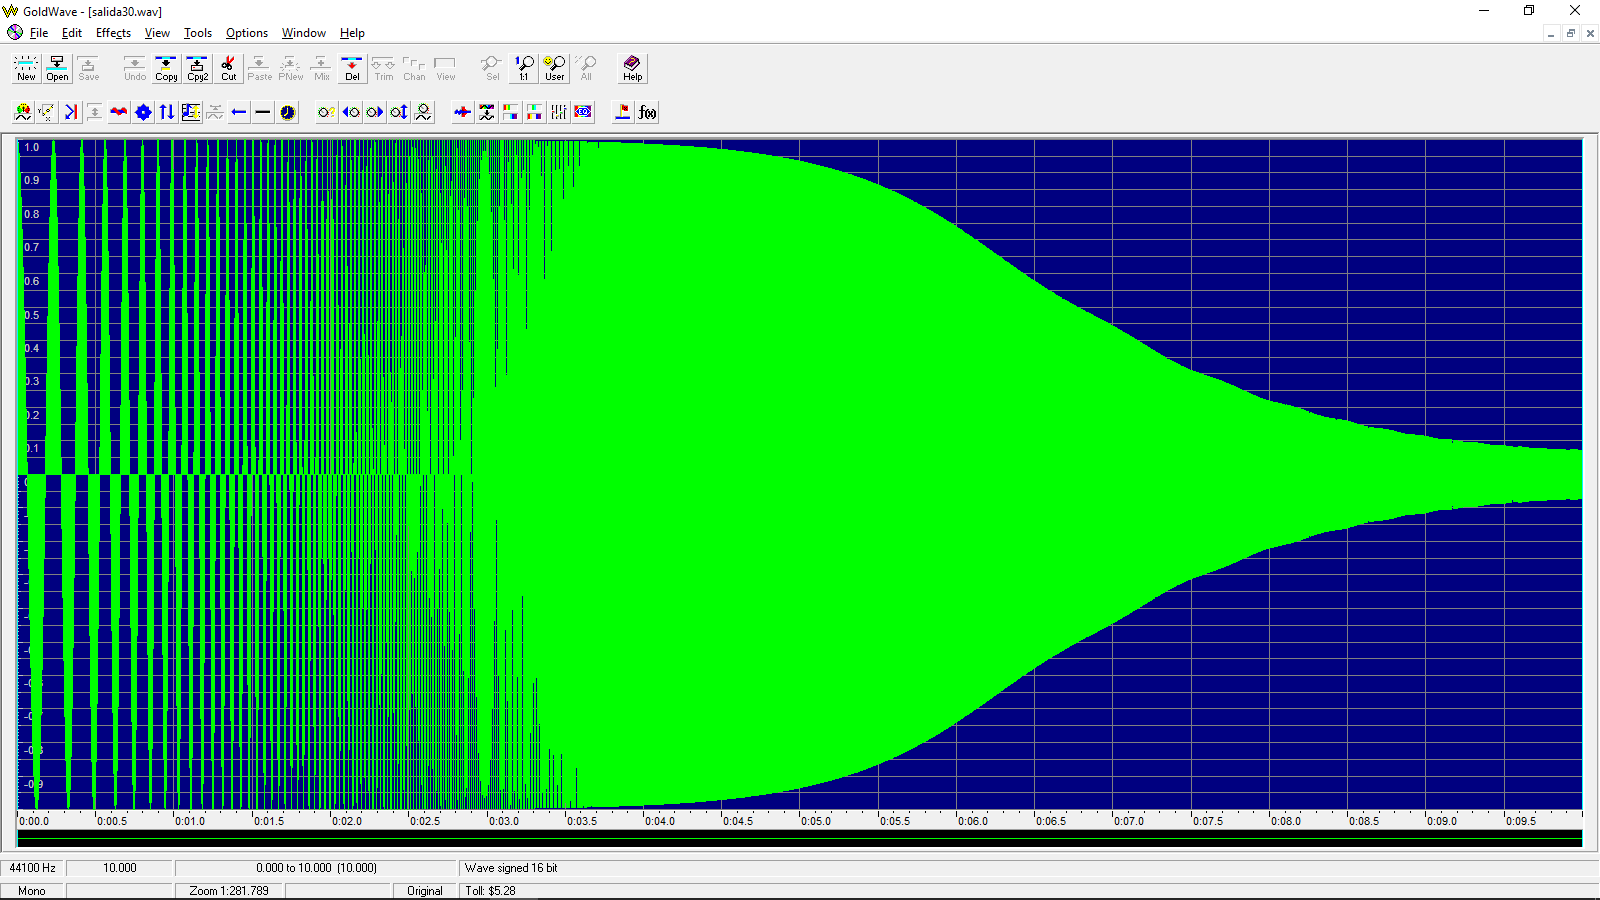
\includegraphics[scale=.28]{img/salida30.png}
	\caption{Salida 1 - 30 coeficientes en el filtro}
	\label{fig:salida30}		
\end{figure}
\begin{figure}[H]
	\centering
	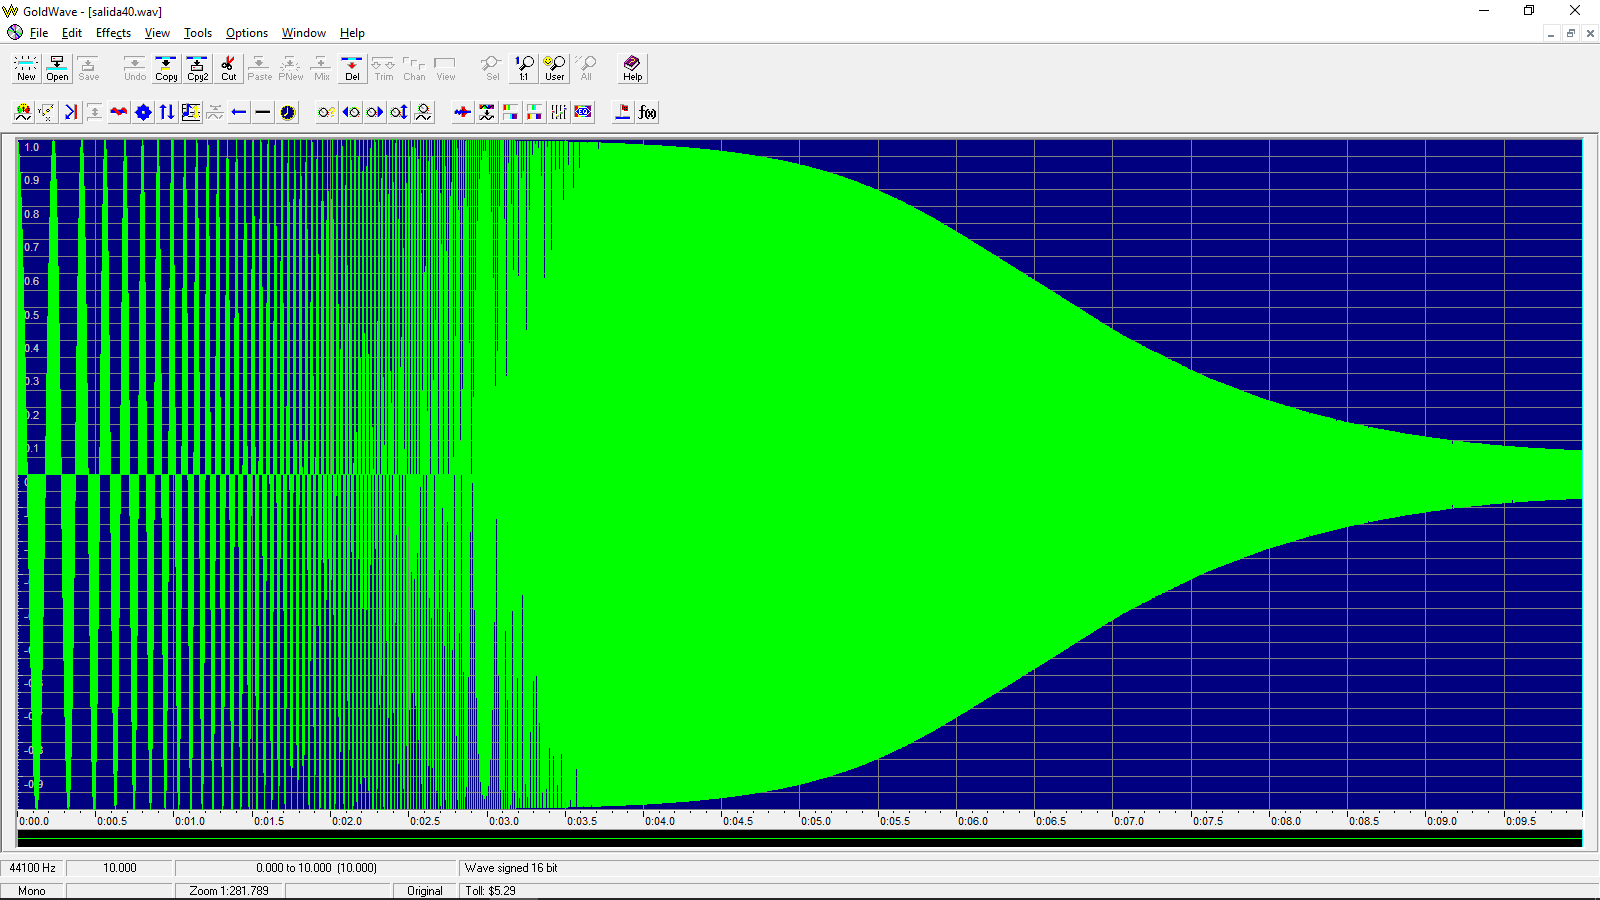
\includegraphics[scale=.28]{img/salida40.png}
	\caption{Salida 1 - 40 coeficientes en el filtro}
	\label{fig:salida30}		
\end{figure}
Como puede observarse en las Figuras 6 y 7, mientras más coeficientes son usados para representar el filtro, este se comporta más como un filtro ideal., debido a que al momento de realizarse la convolución, la señal del filtro cuenta con más puntos, permitiendo así, aumentar la precisión de la convolución.